\documentclass{beamer}
% (fold)
\graphicspath{{./Images/}} % the folder in which images are stored for this project
\usepackage{tikz,graphicx,amsmath,hyperref,tcolorbox,fancyvrb,xcolor}
\hypersetup{colorlinks=true} % make sure our hyperlinks are coloured for visibility
\definecolor{DBlack}{RGB}{35,31,32}
\definecolor{DPurple}{RGB}{126,49,123}
\definecolor{DBlue}{RGB}{0,99,136}

\tcbuselibrary{skins,breakable}
\newenvironment{BGVerbatim}
 {\VerbatimEnvironment
  \begin{tcolorbox}[
    breakable,
    colback=lightgray,
	boxsep=3mm
  ]%
  \begin{Verbatim}}
 {\end{Verbatim}\end{tcolorbox}}

\usecolortheme[RGB={83,13,88}]{structure}
% This is the theme that we are modifying
\usetheme{Boadilla}

% Change the font colour to white on the title page to stand out against the purple
\setbeamercolor{title}{fg=white}
\setbeamerfont{title}{family=\rmfamily}
\setbeamercolor{author}{fg=white}
\setbeamerfont{author}{series=\bfseries}
\setbeamercolor{institute}{fg=white}
\setbeamercolor{date}{fg=white}
\setbeamerfont{date}{series=\bfseries}

% Remove the default ball bullet points in the toc, but keep the numbering
\setbeamertemplate{sections/subsections in toc}[sections numbered]
% Change the item icons to be circles rather than balls
\setbeamertemplate{itemize items}[circle]
% Define blocks to be rounded rectangles with shadows
\setbeamertemplate{blocks}[rounded][shadow=true]

% Turn the @ symbol into character class other
\makeatother
% Modify the footline to get a two part footline with slide numbers
\setbeamertemplate{footline}
{
  \leavevmode%
  \hbox{%
  % Create a box with width of slide, containing current slide and total slides
  \begin{beamercolorbox}[wd=\paperwidth,ht=2.25ex,dp=1ex,center]{section in head/foot}%
    \insertframenumber{} / \inserttotalframenumber\hspace*{1ex}
  \end{beamercolorbox}}%
  \vskip0pt%
}
% Turn the @ symbol back to a letter
\makeatletter

% Remove the default navigation symbols from the bottom of the slides
\setbeamertemplate{navigation symbols}{}
% (end)
\author{Sam Fearn\\{\small 
(s.m.fearn@durham.ac.uk)}}
%\institute[Durham]{Durham University}
\title{An introduction to version control with Git}
\date{November 5\textsuperscript{th}, 2019}

\begin{document}
% (fold)
% --- Start Custom Commands --- %
\renewcommand{\d}[2][]{\ensuremath{\operatorname{d}^{#1}\!{#2}}}
% --- End Custom Commands --- %

%--- the titlepage frame -------------------------%
{
% Draw a purple box for the background of the title slide and add the durham logo at the bottom
\setbeamertemplate{background canvas}{

\begin{tikzpicture}
    \clip (0,0) rectangle (\paperwidth,\paperheight);
    \fill[color=DPurple] (0,0) rectangle (\paperwidth,\paperheight);
\end{tikzpicture}
}

\begin{frame}[plain]
\maketitle
\end{frame}
}

%---Complete Outline--------------------%
\begin{frame}
       \frametitle{Outline}
       \tableofcontents
\end{frame}
% (end)
\section{Introduction} % (fold)
\label{sec:intro}

\begin{frame}{What is Version Control?}
	\begin{itemize}
		\item<1-> A Version Control System (VCS, sometimes also SCMS) is a tool for managing a changing collection of files, allowing you to get back to a particular version at any time.
		\item<2-> E.g. myfile041119.txt, myfile051119.txt, ...
		\item<3-> The method above has many problems, including duplication, naming errors, easy to accidentally overwrite the old file, ...
		\item<4-> Also, if you're collaborating on a project, this can get very tricky to manage. Which version did I last send? Have I included the latest changes from my collaborator? What do I do if they make changes to a section I've also changed since we last compared?
	\end{itemize}
	\onslide<5->{\center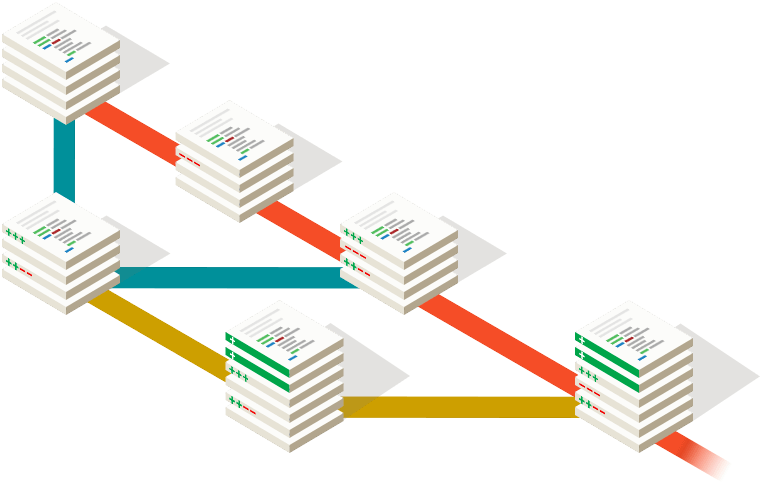
\includegraphics[width=0.4\textwidth]{VC}}
\end{frame}

\begin{frame}{Different VCS}
	\begin{itemize}
		\item<1-> Many different VCS have been created to address the challenges of managing different versions of files.
		\item<2-> Most of the popular systems in use today are either \textbf{Centralised Version Control Systems}, or \textbf{Distributed Version Control Systems}.
		\item<3-> With a CVCS, there is a single server which manages the versioned files -- the main downside is that this type of system has a single point of failure.
		\item<4-> Examples of CVCS you may have heard of include SVN and Subversion.
		\item<5-> In a DVCS, the entire history of each project is mirrored across multiple clients -- this protects against the single point of failure.
		\item<6-> Common examples of DVCS include Git and Mercurial.
		\item<7-> Of all the systems mentioned above, Git is probably the most common and widely used.
	\end{itemize}
	\onslide<8->{\center
\includegraphics[width=0.1\textwidth]{gitlogo}}
\end{frame}

\begin{frame}{Git and Github}
	\onslide<1->{\center
\includegraphics[width=0.5\textwidth]{Octocat}}
	\begin{itemize}
		\item<1-> Github is a free git hosting service, allowing you to share repositories with other people (or keep them private) -- alternatives do exist (Bitbucket, Kiln?).
		\item<2-> Git can be used without Github. Your repository is always stored locally, and you can share this however you wish -- ssh, ftp, (email, memory stick,...!) etc.
	\end{itemize}
\end{frame}

% section intro (end)

\section{How to actually use git} % (fold)
\label{sec:how_to_actually_use_git}
\begin{frame}[fragile]{Using Git at the command line}
	Creating a new repository
	\begin{itemize}
		\item<1-> \verb|git init|
	\end{itemize}
	\onslide<2->{\textbf{Cloning} an existing repository}
	\begin{itemize}
		\item<2-> \verb|git clone username@host:/path/to/repository|
	\end{itemize}
	\onslide<3->{Check the \textbf{status} of a repository}
	\begin{itemize}
		\item<3-> \verb|git status|
	\end{itemize}
	\onslide<4->{\textbf{Add} files to the index}
	\begin{itemize}
		\item<4-> \verb|git add filename|
		\item<5-> Or \verb|git add *|
		\item<6-> Or \verb|git add -u|
	\end{itemize}
	\onslide<7->{ \textbf{Commit} the changes}
	\begin{itemize}
		\item<7-> \verb|git commit -m "Helpful message"|
	\end{itemize}
	\onslide<8->{ \textbf{Add a remote} server (if neccessary)}
	\begin{itemize}
		\item<8-> \verb|git remote add origin <server>|
	\end{itemize}
	\onslide<9->{ \textbf{Push} the recent commits}
	\begin{itemize}
		\item<9-> \verb|git push origin master|
	\end{itemize}
\end{frame}

\begin{frame}[fragile]{What's going on?}
	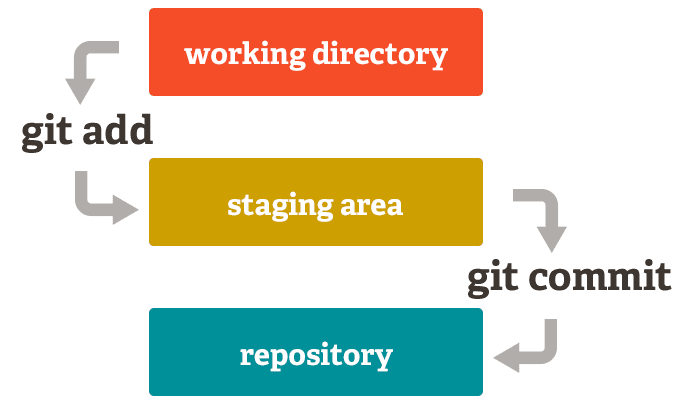
\includegraphics[width=\textwidth]{gitstaging}
\end{frame}

\begin{frame}[fragile]{Updating to new changes}
	\onslide<1->{To update to the most recent commit}
	\begin{itemize}
		\item<1-> \verb|git pull|
	\end{itemize}
	\onslide<2->{This syncs the local repository with the remote one, automatically merging changes}
	\medskip
	\onslide<3->{What if we want to work on different things at the same time?}
	\onslide<4->{Create a new \textbf{branch}}
	\begin{itemize}
		\item<4-> \verb|git checkout -b <branch>|
	\end{itemize}
	\onslide<5->{After making some changes, \textbf{push} branch}
	\begin{itemize}
		\item<5-> \verb|git push origin <branch>|
	\end{itemize}
	\onslide<6->{Switch between branches}
	\begin{itemize}
		\item<6-> \verb|git checkout <branch>|
	\end{itemize}
	\onslide<7->{\textbf{Merge} a branch into the current branch}
	\begin{itemize}
		\item<6-> \verb|git merge <branch>|
	\end{itemize}
\end{frame}

\begin{frame}[fragile]{What's going on 2?}
	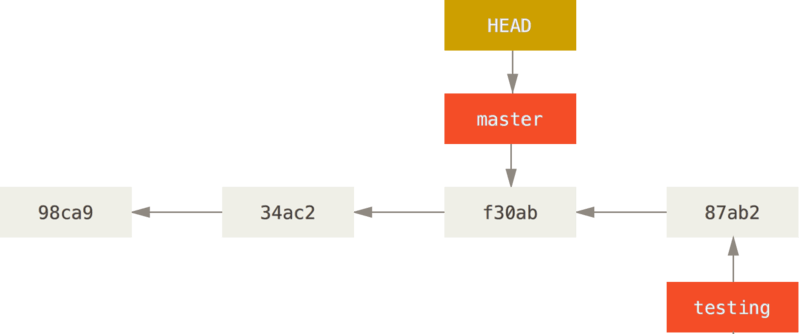
\includegraphics[width=\textwidth]{gitbranches}
\end{frame}

\begin{frame}{Git GUIs}
	Sorry, I was going to demo, I ran out of time. The following are cross-platform.
	\begin{itemize}
		\item Github Desktop
		\item Fork
	\end{itemize}
\end{frame}
% section how_to_actually_use_git (end)

\section{Useful Resources} % (fold)
\label{sec:useful_resources}
\begin{frame}{Useful Resources}
	 \begin{itemize}
	 	\item \href{https://rogerdudler.github.io/git-guide/}{Git - the simple guide}
	 	\item \href{https://book.git-scm.com}{The Git Community Book}
	 	\item \href{https://rogerdudler.github.io/git-guide/files/git_cheat_sheet.pdf}{Git Cheatsheet}
	 \end{itemize}
\end{frame}
% section useful_resources (end)

\end{document}